\documentclass[tikz]{standalone}
\usetikzlibrary{arrows, positioning}
\begin{document}
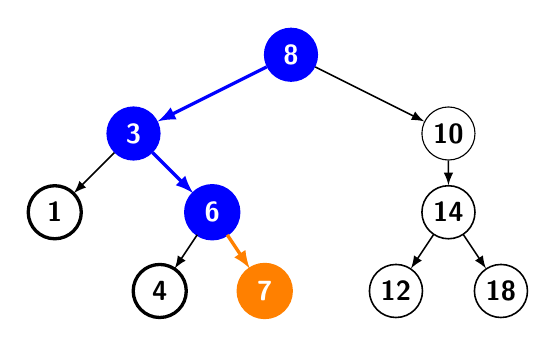
\begin{tikzpicture}[level/.style={sibling distance = 4cm/#1,
  level distance = 1cm},
  treenode/.style = {align=center, inner sep=1pt, text centered,
  font=\sffamily},
bst/.style = {treenode, circle, black, font=\sffamily\bfseries, draw=black, text width=1.5em},
bluebst/.style = {treenode, circle, white, font=\sffamily\bfseries, draw=blue, fill=blue, text width=1.5em},
orangebst/.style = {treenode, circle, white, font=\sffamily\bfseries, draw=orange, fill=orange, text width=1.5em},
blueline/.style={edge from parent/.style={blue,very thick,-latex,draw}},
orangeline/.style={edge from parent/.style={orange,very thick,-latex,draw}},
commonline/.style={edge from parent/.style={black,line width=0.2mm,-latex,draw}},
]
\node [bluebst] {8}
    child[blueline] {node [bluebst] {3}
        child[commonline] {node [bst] {1}}
        child {node [bluebst] {6}
            child[commonline] {node [bst] {4}}
            child[orangeline] {node [orangebst] {7}}
        }
    }
    child[commonline] {node [bst] {10}
        child {node [bst] {14}
            child {node [bst] {12}}
            child {node [bst] {18}}
        }
    }
;
\end{tikzpicture}
\end{document}
